%!TEX root = ../Thesis.tex

\section{Incorporating Error}
The error was systematically added in a randomly uniform fashion in three types of ways; satellite correlated error, receiver correlated error and random error. A statistically significant sample size of 100 iterations was conducted with the simulation using error created in Eq\eqref{Eq: errorstruc}. The planar algorithm was compared to NLLS using the same errors for each iteration. The mean and standard deviation were calculated. The satellite configuration for this section was Figure \ref{fig:satconfig_1m}.\\

The planar algorithm (PA) worked very well for satellite correlated errors, confirming the differential method of removing correlated errors, see Figure \ref{fig:Error_satellite}. The error for PA was consistent at $10^{-6}$ m, this lower limit was observed previously and is a product of the clock bias solution. Relative NLLS error increased linearly with the satellite correlated errors until it reached numerical instability.\\

PA also worked well at removing receiver correlated errors with an error of $10^{-6}$ m, however NLLS had better performance, see Figure \ref{fig:Receivers}. Large errors of $>10^{-3}$ seconds, which corresponds to a pseudorange error of $10^{-3}c = 298\; km$ might have the planar assumption effecting the solution.\\

Uncorrelated errors had the worst affect on the system, see Figure \ref{fig:Uncorellated}. But PA performed just as well as NLLS with error proportional to $c\times t$. This was expected as PA is based on removing errors by linear difference.

\begin{figure}
\centering
\caption{An Ideal Satellite Configuration for Northerly Displaced Receivers}
\label{fig:satconfig_1m}
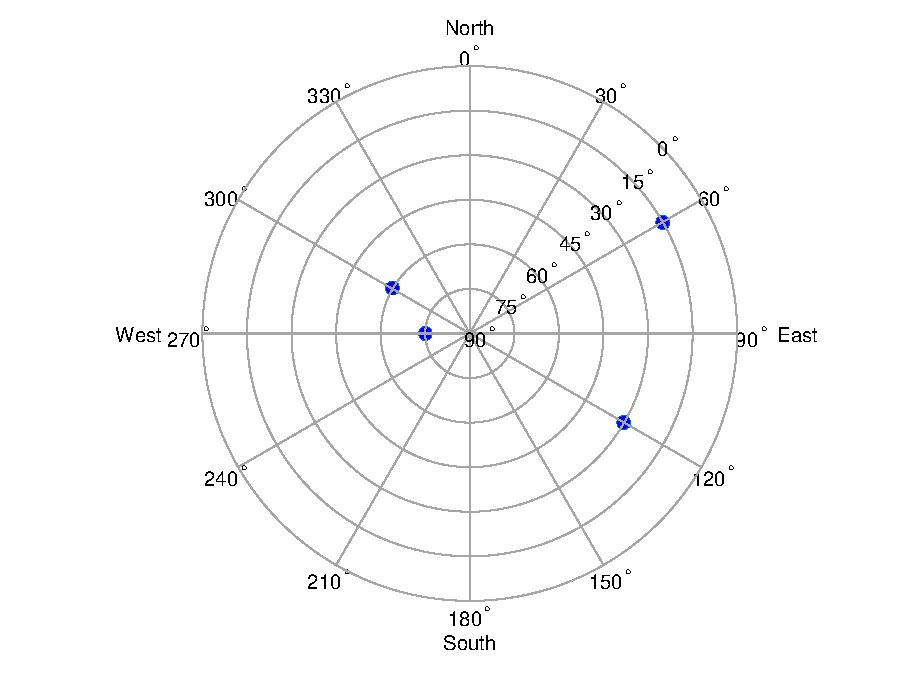
\includegraphics[width=0.7\linewidth]{ChapterExperiments/Figures/ControlledError/satconfig_1m}
\end{figure}


\begin{figure}
\centering
\caption{}
\label{fig:Error_satellite}
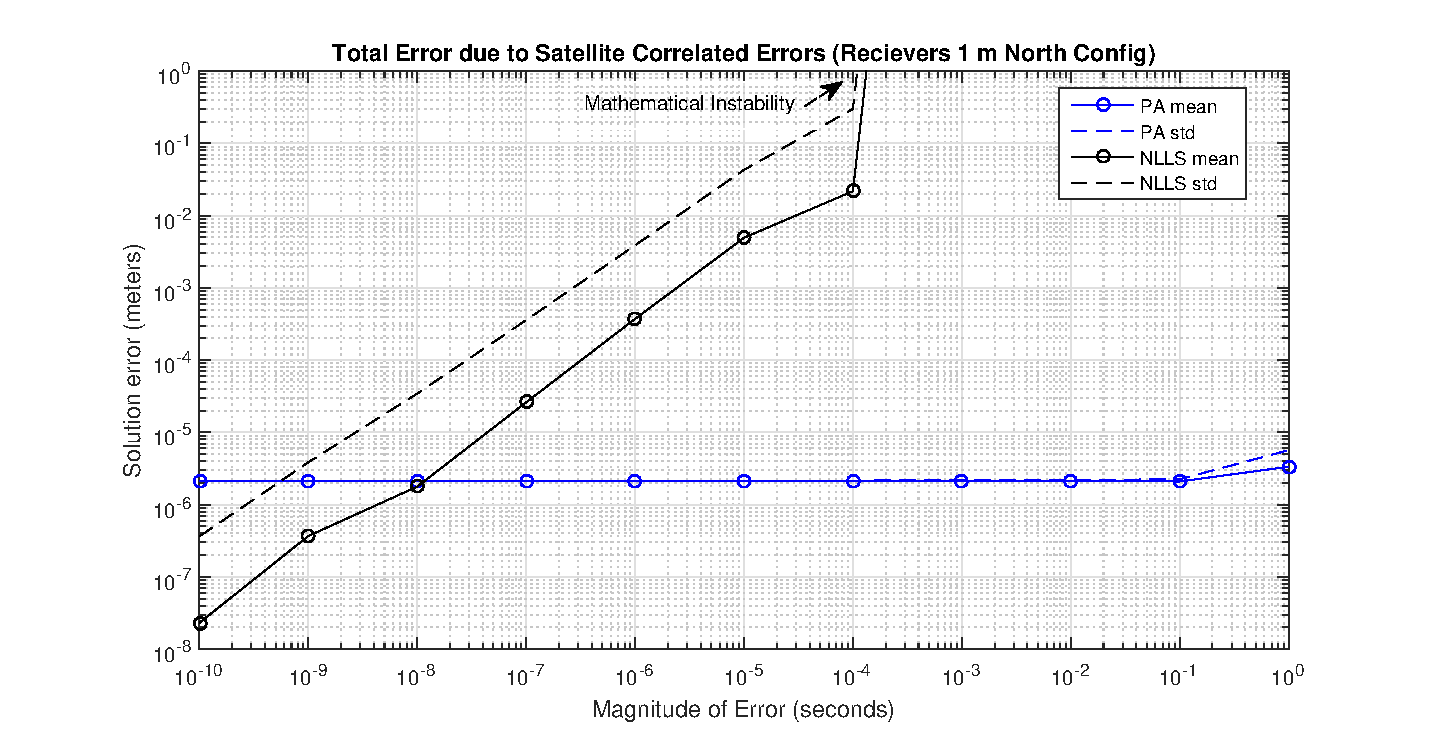
\includegraphics[width=1\linewidth]{ChapterExperiments/Figures/ControlledError/satellite}
\end{figure}

\begin{figure}
\centering
\caption{}
\label{fig:Receivers}
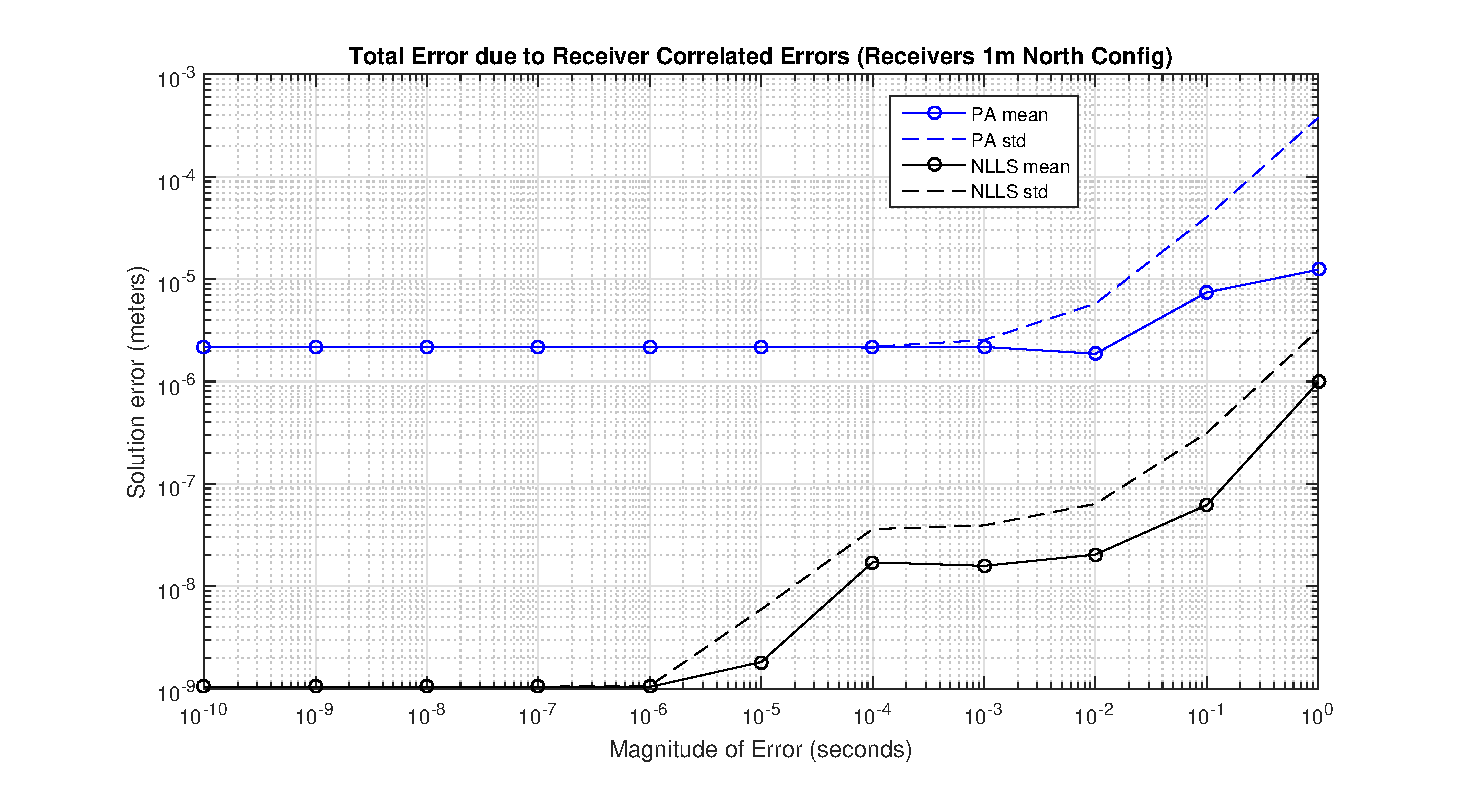
\includegraphics[width=1\linewidth]{ChapterExperiments/Figures/ControlledError/Receivers}
\end{figure}
\begin{figure}
\centering
\caption{}
\label{fig:Uncorellated}
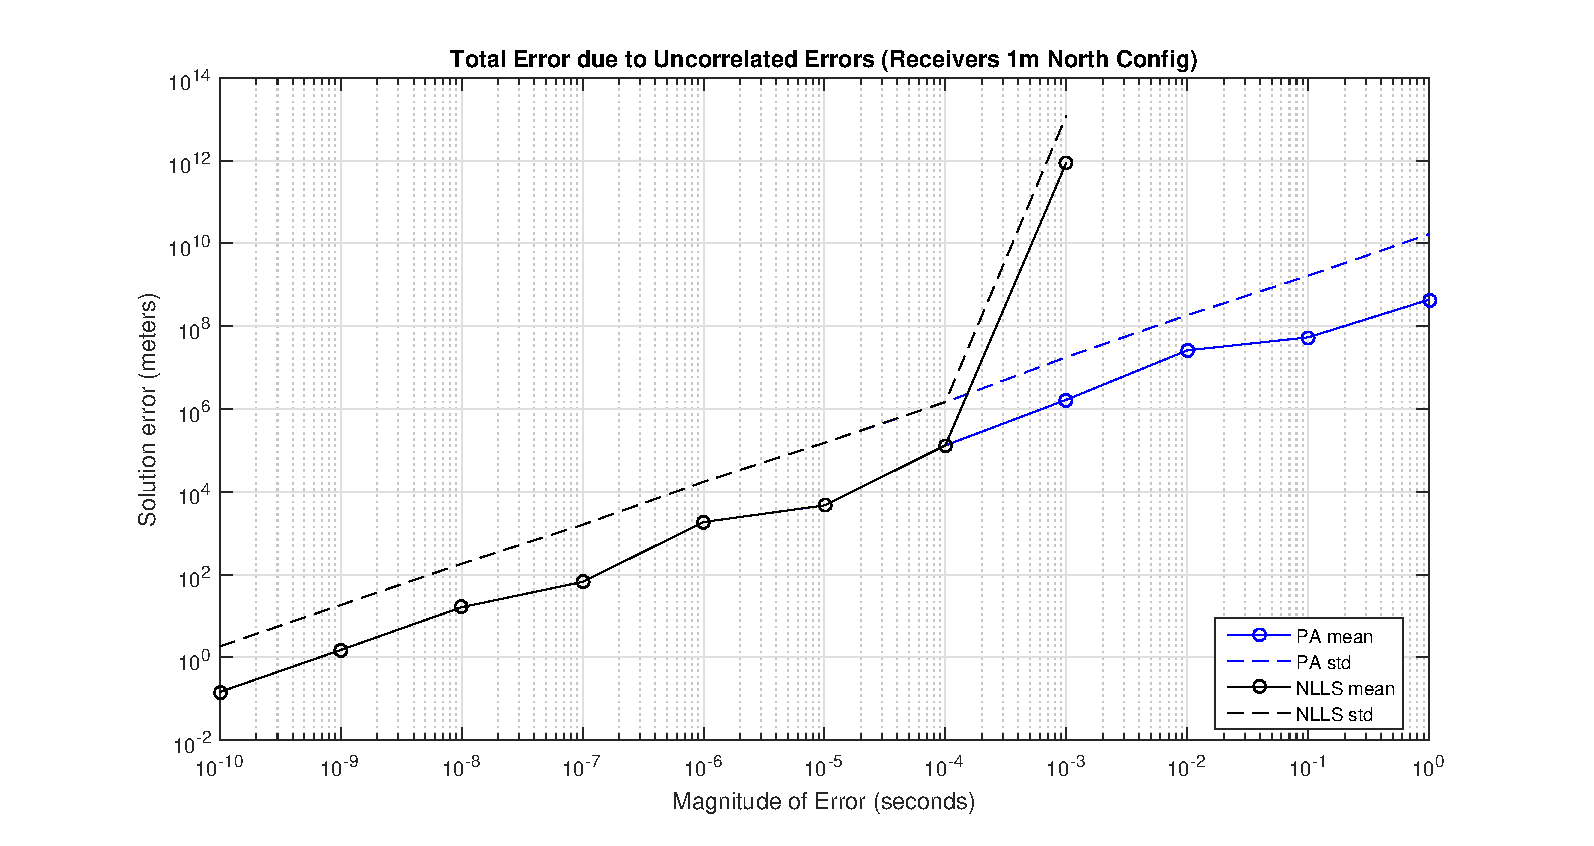
\includegraphics[width=1\linewidth]{ChapterExperiments/Figures/ControlledError/Uncorellated}
\end{figure}


